\documentclass[border=5mm]{standalone}
\usepackage{tikz}
\usetikzlibrary{arrows.meta,positioning,calc}
\usepackage{times}

\begin{document}
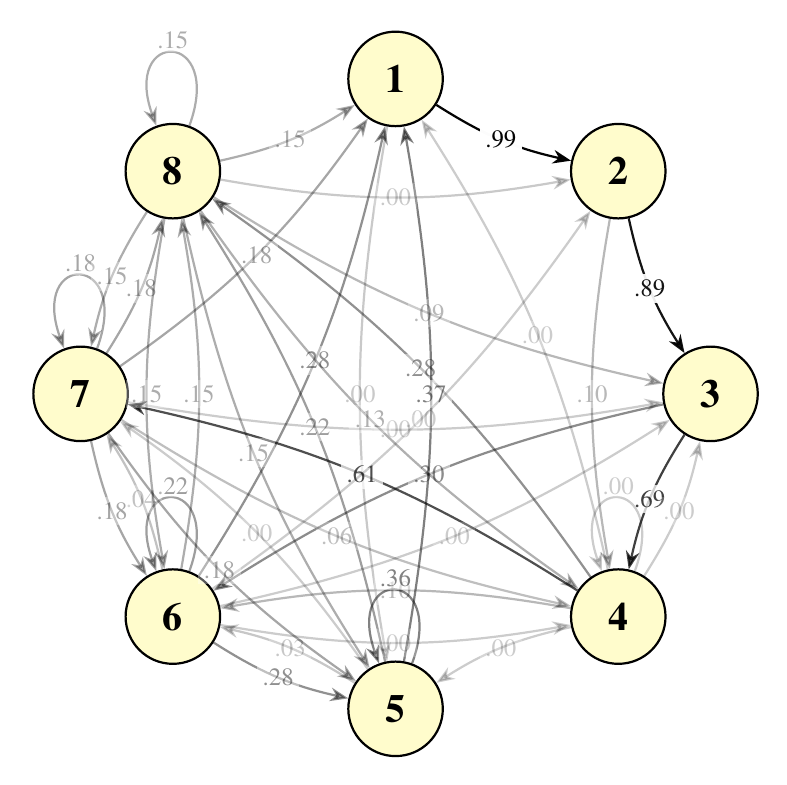
\begin{tikzpicture}[
    node distance=3cm,
    state/.style={circle, draw=black, thick, minimum size=1.2cm, fill=yellow!20, font=\Large\bfseries\fontfamily{ptm}\selectfont},
    every edge/.style={draw, thick, -Stealth},
    edge label/.style={font=\small\fontfamily{ptm}\selectfont, black, fill=white, inner sep=1pt}
]

\node[state] (1) at (90.0:4cm) {1};
\node[state] (2) at (45.0:4cm) {2};
\node[state] (3) at (0.0:4cm) {3};
\node[state] (4) at (-45.0:4cm) {4};
\node[state] (5) at (-90.0:4cm) {5};
\node[state] (6) at (-135.0:4cm) {6};
\node[state] (7) at (-180.0:4cm) {7};
\node[state] (8) at (-225.0:4cm) {8};

\path (1) edge[bend right=10, opacity=0.99] node[edge label, midway, fill=white, inner sep=2pt] {.99} (2);
\path (1) edge[bend right=10, opacity=0.21] node[edge label, midway, fill=white, inner sep=2pt] {.00} (5);
\path (2) edge[bend right=10, opacity=0.92] node[edge label, midway, fill=white, inner sep=2pt] {.89} (3);
\path (2) edge[bend right=10, opacity=0.28] node[edge label, midway, fill=white, inner sep=2pt] {.10} (4);
\path (3) edge[bend right=10, opacity=0.75] node[edge label, midway, fill=white, inner sep=2pt] {.69} (4);
\path (3) edge[bend right=10, opacity=0.45] node[edge label, midway, fill=white, inner sep=2pt] {.30} (6);
\path (4) edge[bend right=10, opacity=0.20] node[edge label, midway, fill=white, inner sep=2pt] {.00} (1);
\path (4) edge[bend right=10, opacity=0.20] node[edge label, midway, fill=white, inner sep=2pt] {.00} (3);
\path (4) edge[loop, out=70, in=110, looseness=8, opacity=0.20] node[edge label, above] {.00} (4);
\path (4) edge[bend right=10, opacity=0.20] node[edge label, midway, fill=white, inner sep=2pt] {.00} (5);
\path (4) edge[bend right=10, opacity=0.28] node[edge label, midway, fill=white, inner sep=2pt] {.10} (6);
\path (4) edge[bend right=10, opacity=0.69] node[edge label, midway, fill=white, inner sep=2pt] {.61} (7);
\path (4) edge[bend right=10, opacity=0.43] node[edge label, midway, fill=white, inner sep=2pt] {.28} (8);
\path (5) edge[bend right=10, opacity=0.50] node[edge label, midway, fill=white, inner sep=2pt] {.37} (1);
\path (5) edge[loop, out=70, in=110, looseness=8, opacity=0.49] node[edge label, above] {.36} (5);
\path (5) edge[bend right=10, opacity=0.22] node[edge label, midway, fill=white, inner sep=2pt] {.03} (6);
\path (5) edge[bend right=10, opacity=0.20] node[edge label, midway, fill=white, inner sep=2pt] {.00} (7);
\path (5) edge[bend right=10, opacity=0.38] node[edge label, midway, fill=white, inner sep=2pt] {.22} (8);
\path (6) edge[bend right=10, opacity=0.43] node[edge label, midway, fill=white, inner sep=2pt] {.28} (1);
\path (6) edge[bend right=10, opacity=0.20] node[edge label, midway, fill=white, inner sep=2pt] {.00} (2);
\path (6) edge[bend right=10, opacity=0.20] node[edge label, midway, fill=white, inner sep=2pt] {.00} (3);
\path (6) edge[bend right=10, opacity=0.20] node[edge label, midway, fill=white, inner sep=2pt] {.00} (4);
\path (6) edge[bend right=10, opacity=0.43] node[edge label, midway, fill=white, inner sep=2pt] {.28} (5);
\path (6) edge[loop, out=70, in=110, looseness=8, opacity=0.38] node[edge label, above] {.22} (6);
\path (6) edge[bend right=10, opacity=0.24] node[edge label, midway, fill=white, inner sep=2pt] {.04} (7);
\path (6) edge[bend right=10, opacity=0.32] node[edge label, midway, fill=white, inner sep=2pt] {.15} (8);
\path (7) edge[bend right=10, opacity=0.35] node[edge label, midway, fill=white, inner sep=2pt] {.18} (1);
\path (7) edge[bend right=10, opacity=0.20] node[edge label, midway, fill=white, inner sep=2pt] {.00} (3);
\path (7) edge[bend right=10, opacity=0.25] node[edge label, midway, fill=white, inner sep=2pt] {.06} (4);
\path (7) edge[bend right=10, opacity=0.35] node[edge label, midway, fill=white, inner sep=2pt] {.18} (5);
\path (7) edge[bend right=10, opacity=0.35] node[edge label, midway, fill=white, inner sep=2pt] {.18} (6);
\path (7) edge[loop, out=70, in=110, looseness=8, opacity=0.35] node[edge label, above] {.18} (7);
\path (7) edge[bend right=10, opacity=0.35] node[edge label, midway, fill=white, inner sep=2pt] {.18} (8);
\path (8) edge[bend right=10, opacity=0.32] node[edge label, midway, fill=white, inner sep=2pt] {.15} (1);
\path (8) edge[bend right=10, opacity=0.21] node[edge label, midway, fill=white, inner sep=2pt] {.00} (2);
\path (8) edge[bend right=10, opacity=0.28] node[edge label, midway, fill=white, inner sep=2pt] {.09} (3);
\path (8) edge[bend right=10, opacity=0.31] node[edge label, midway, fill=white, inner sep=2pt] {.13} (4);
\path (8) edge[bend right=10, opacity=0.32] node[edge label, midway, fill=white, inner sep=2pt] {.15} (5);
\path (8) edge[bend right=10, opacity=0.32] node[edge label, midway, fill=white, inner sep=2pt] {.15} (6);
\path (8) edge[bend right=10, opacity=0.32] node[edge label, midway, fill=white, inner sep=2pt] {.15} (7);
\path (8) edge[loop, out=70, in=110, looseness=8, opacity=0.32] node[edge label, above] {.15} (8);

\end{tikzpicture}
\end{document}
